%% Autor: Björn Ritterbecks 
%% Letzte Aenderung: 15.06.2016 
\thisfloatsetup{%
  capbesidewidth=\marginparwidth}
\begin{figure}[htbp]
\vspace*{0.2cm}
\centering
%\sansmath
 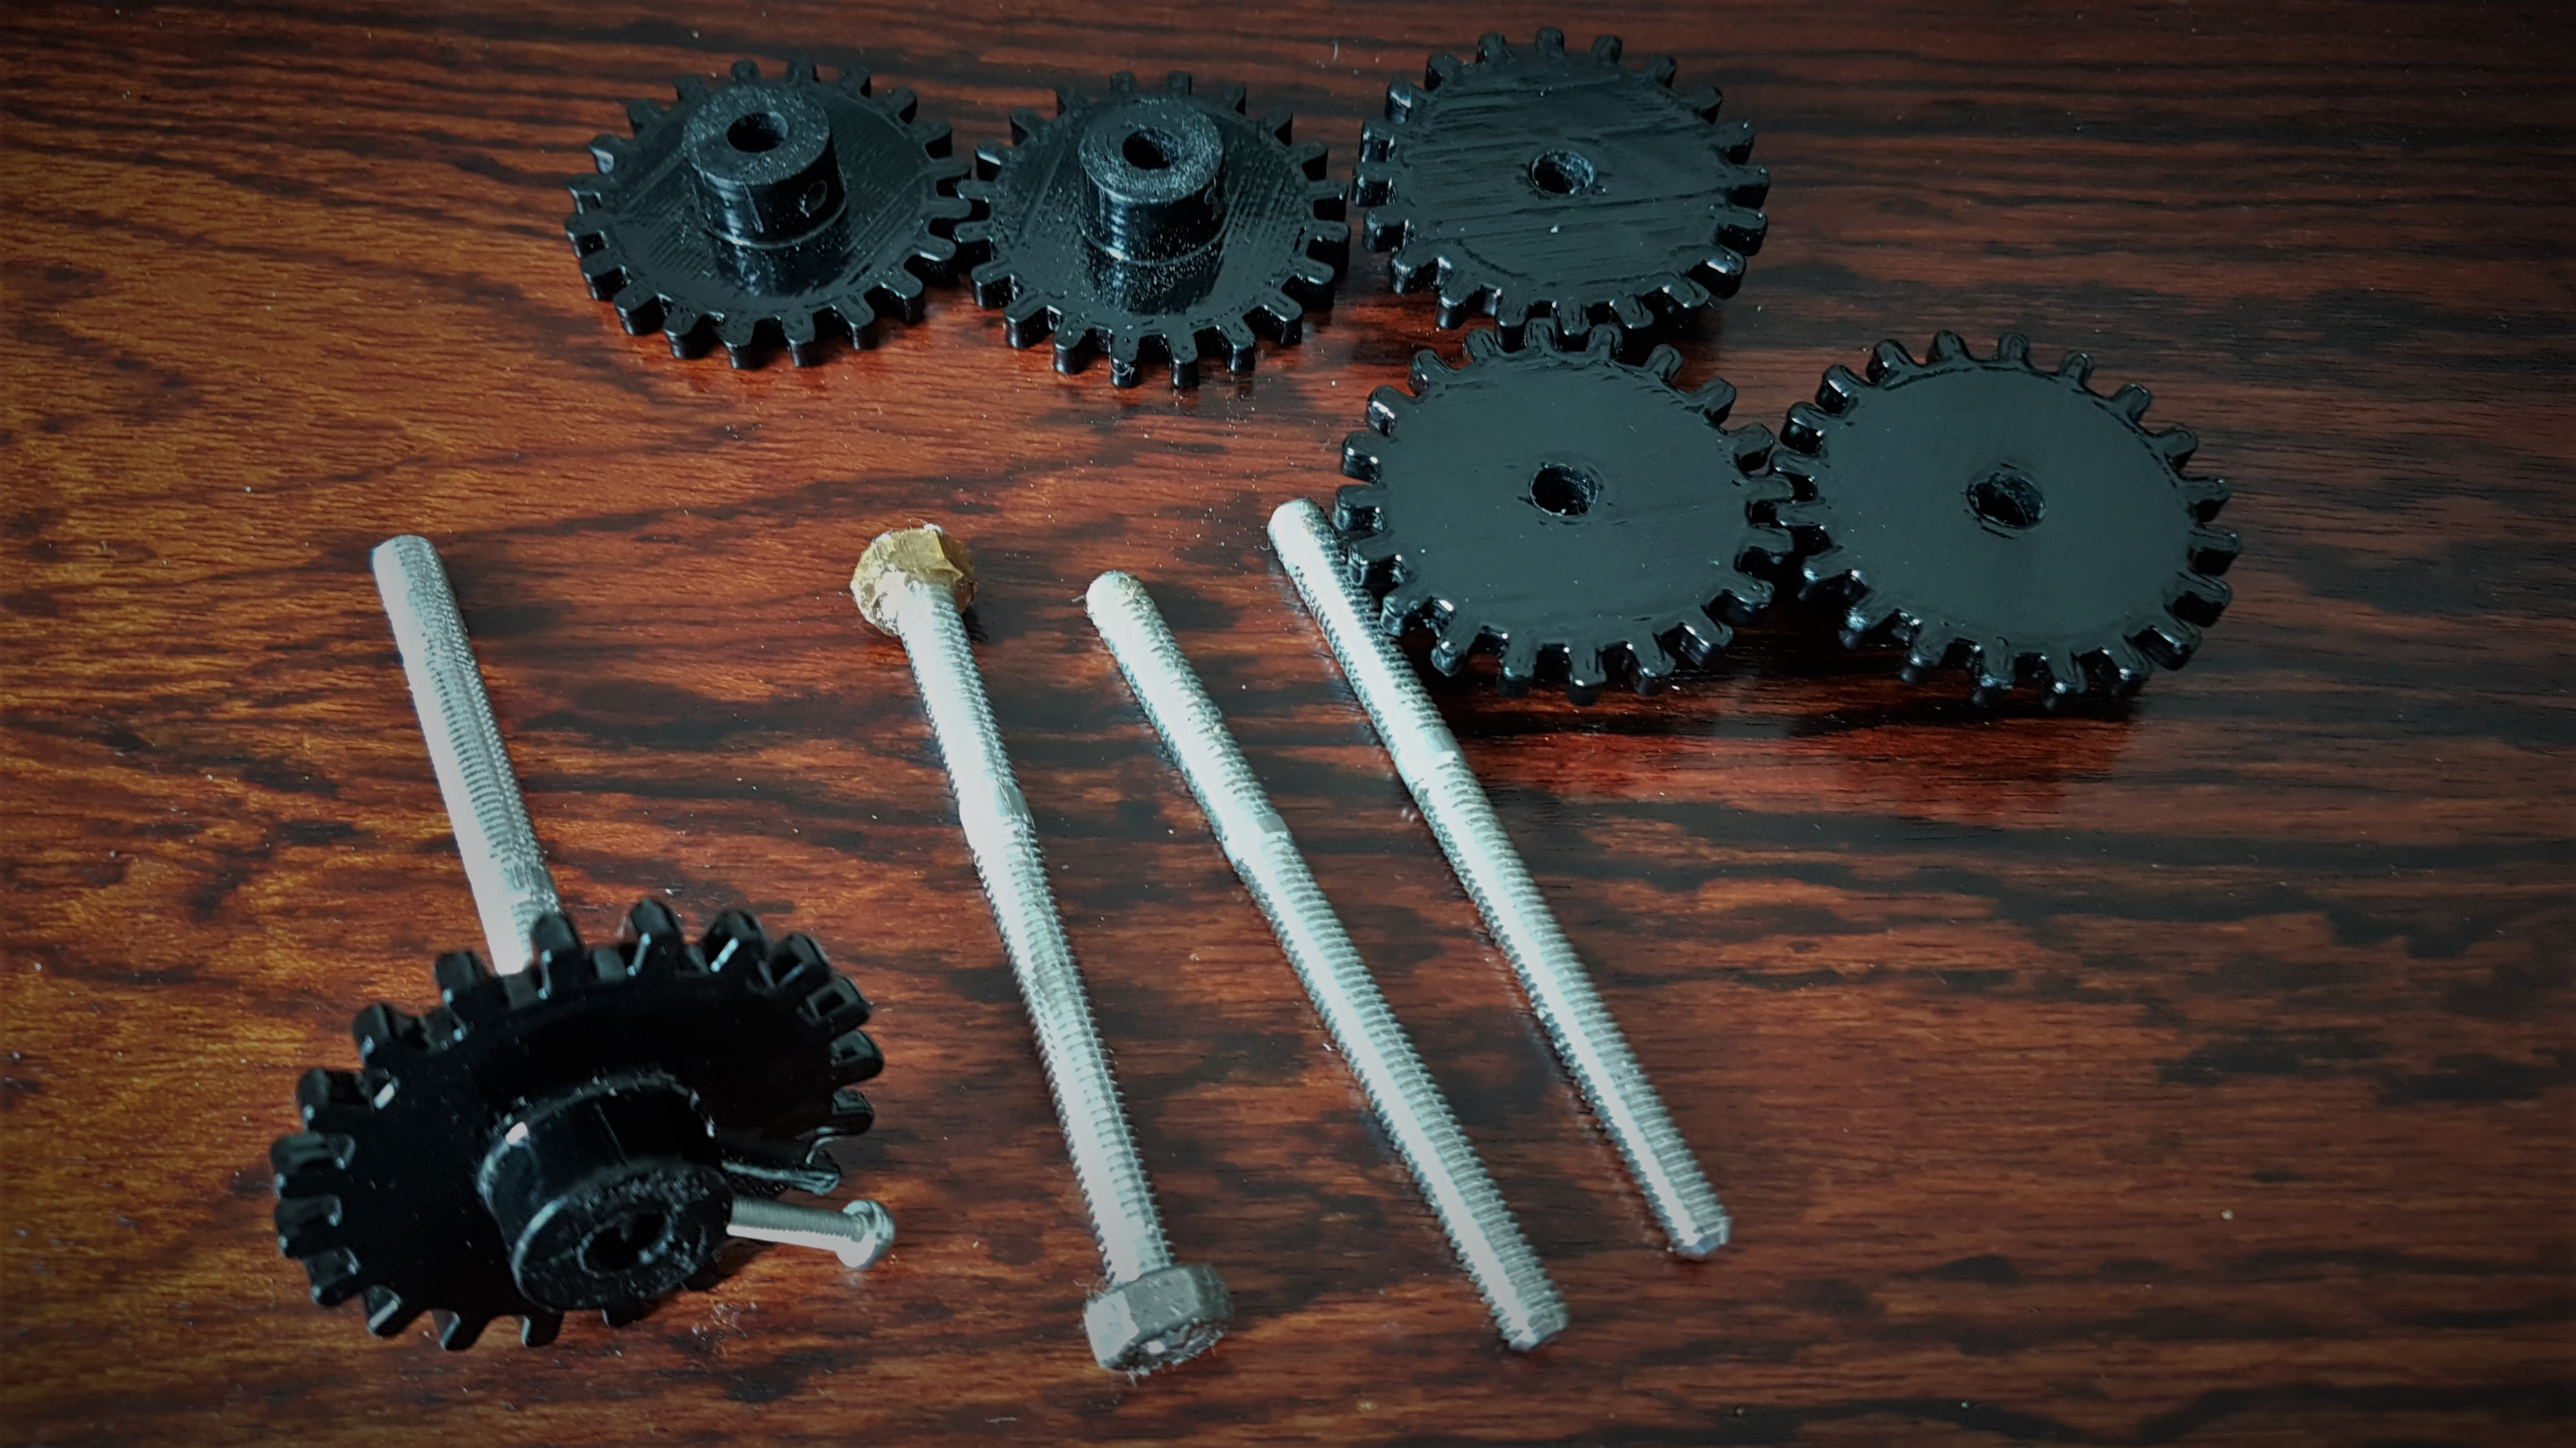
\includegraphics[width=0.99\textwidth]{images/toothpaste.jpg}
  \caption[Fotografie der Zahnräder und Gewinde]{Fotografische Abbildung der Zahnräder und Gewinde nach dem Ausbau. Bei Versuchen vor dem Einkleben der Muttern haben beide Komponenten gut funktioniert, wurden jedoch bei der Arretierung an der Beschleunigereinheit in ihrer Funktionalität zerstört (unter anderem durch Kleberückstände und mangelhafte Parallelität).}
  \label{fig:toothpaste}
  \vspace{-0pt}
\end{figure}